\documentclass[11pt]{article}

\usepackage{amsmath,amssymb,amsthm,amsfonts,graphicx,cite,mathrsfs,upgreek}

\newtheorem{theorem}{Theorem}
\newtheorem{definition}{Definition}
\newcommand{\pare[1]}{\left( #1 \right)}
\newcommand{\R}{\ensuremath{\mathbb{R}}}
\newcommand{\Z}{\ensuremath{\mathbb{Z}}}
\newcommand{\Q}{\ensuremath{\mathbb{Q}}}

\begin{document}

\title{A Brief Survey of Elliptic Curve Public Key Cryptosystem}
\author{Seongjin Cho (Josh)}

\maketitle

\tableofcontents

\newpage

\section{Introduction}
The development of an elliptic curve both strengthened the security and increased the performance of public key cryptosystems because it enabled us to use a smaller key size in approximately same degree of security. However, one may naturally ask how this seemingly unrelated object \emph{elliptic curve} plays an active role in public key cryptosystems. To answer this question, this paper will investigate what properties of the elliptic curve enabled such a strong security. Also, this paper will further discuss a specific example key agreement protocol called \emph{Elliptic curve Diffie-Hellman} (ECDH). Much of our the work in this paper is based on Professor William Stein’s \emph{Elementary Number Theory}~\cite{Stein} and Professor Neal Koblitz's  \emph{A Course in Number Theory and Cryptography}~\cite{Neal}.

We will first introduce some terminologies and background information about the public key cryptography. We then briefly define and enumerate several properties of an elliptic curve to emphasize certain aspects that improved previous cryptosystems. Next, We will conclude our paper with currently common cryptosystem called Elliptic curve Diffie-Hellman using analogue between Alice and Bob.


\section{Some Background Knowledge}
Before the public key cryptography, symmetric cryptosystems had been used for secure communications. A public key cryptosystem was first introduced by W.Diffie and M.Hellman in 1976. Unlike traditional symmetric cryptosystems, the public key cryptosystem has a property that even though someone knows how to encrypt the message, he or she cannot decrypt the message in reasonable amount of time. The concept of public key cryptosystem is closely related to the one-way function. This is a function which is easy to compute but for which its inverse is very hard to compute.

One most important and useful property of a public key cryptosystem is that a secure communication is possible between two parties without ever having to arrange prior meeting or trust each other. Every information needed for communication is available publicly.

\begin{figure}[t]
\centering
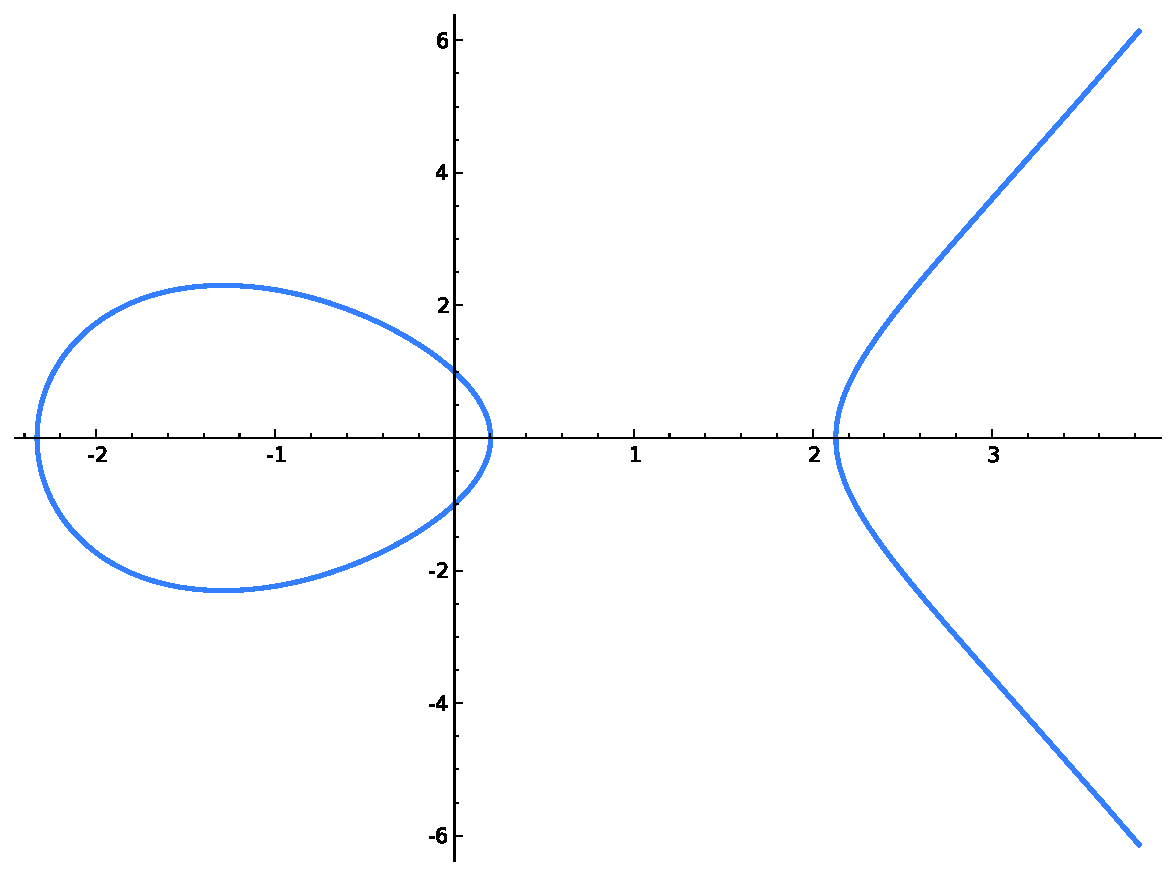
\includegraphics[width=0.5\textwidth]{2.pdf}
\caption{$y^2 = x^3 - 5x + 1$}
\end{figure}

\section{Elliptic curve}
\begin{definition}
An elliptic curve over a field $K$ is a curve defined by an equation of the form 
\begin{equation}
y^2 = x^3+ax+b \label{eq:elliptic}
\end{equation}
where $a,b \in K$ and $4a^3 + 27b^2 \ne 0$.
\end{definition}
The condition that $4a^2 + 27b^2 \ne 0$ guarantees us to have no singular points. If $K$ has characteristic $2$ or $3$, for any choice of $a,b$ will cause $4a^2 + 27b^2$ to be $0$. But, the definition of elliptic curve can be generalized to a form
$$y^2 + a_1xy + a_3y = x^3 + a_2x^2 + a_4x + a_6.$$
This equation correctly allows for elliptic curves in characteristic $2$ and $3$. However, we will use the form~(\ref{eq:elliptic}) mostly in this paper.

\begin{figure}[h]
\centering
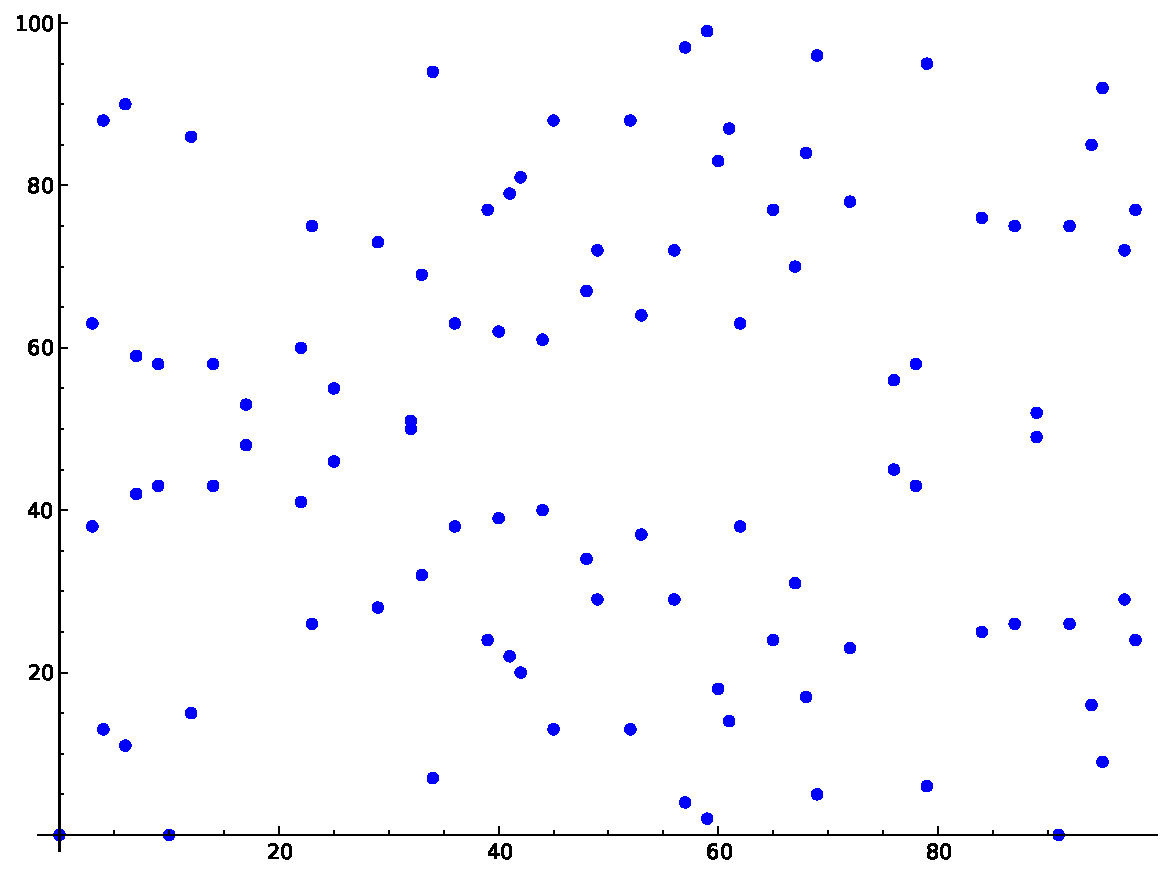
\includegraphics[width=0.5\textwidth]{1.pdf}
\caption{$y^2 = x^3 + x$ over $F_{101}$}
\end{figure}

\subsection{Points on the elliptic curve}
One of the most important properties of an elliptic curve is that the points on the elliptic curve form an abelian group. To explain this more visually, we will assume for now that $K = \R$. We will first prove that the line which crosses two points on the elliptic curve has one more point of intersection on the elliptic curve. We will allow ourselves to consider the point at infinity as a special point on the curve.
\begin{theorem}
Suppose $P = (x_1, y_1)$ and $Q = (x_2, y_2)$ are distinct points on an elliptic curve $y^2 = x^3 + ax + b$, and that $x_1 \ne x_2$. Let $l$ be the unique line through $P$ and $Q$. Then $l$ intersects the graph of $E$ at exactly one other point
$$R = (m^2 - x_1 - x_2, mx_3 + \upnu),$$
where $m = (y_1-y_2)/(x_1-x_2)$ and $\upnu = y_1 - mx_1$.
\end{theorem}
\begin{proof}
We have the line $l = m(x - x_1) + y_1$. Substituting this into the equation~(\ref{eq:elliptic}), we have
$$(m(x - x_1) + y_1)^2 = x^3 + ax + b.$$
Some simplification gives us $f(x) = x^3 - m^2x^2 + \cdots = 0$ which is an cubic equation. Then, by Fundamental Theorem of Algebra, it has three roots including multiple roots. But since $x_1$ and $x_2$ are already on the elliptic curve, it is roots of this cubic equation, so we have $f(x) = (x-x_1)(x-x_2)(x-x_3) = 0$. We can see that $x_1 + x_2 + x_3 = m^2$. Thus $x_3 = m^2 - x_1 - x_2$, as claimed. Also, we can calculate $\upnu$ easily because $y_3 = m(x_3 - x_1) + y_1 = mx_3 + \upnu$.
\end{proof}


Using this theorem, we define a binary operation $+$.
\begin{definition}
Let $E$ be an elliptic curve over the real numbers, and let $P$ and $Q$ be two points on $E$. We define the negative $P$ and the sum $P+Q$ according to the following rules:
\begin{enumerate}
\item If $P$ is the point at infinity $O$, then we define $-P$ to be $O$ and $P+Q$ to be $Q$; that is, $O$ serves as the additive identity of the group of points. For next rules, we shall suppose that neither $P$ or $Q$ is the point at infinity.
\item The negative $-P$ is the point with the same $x$-coordinate but negative the $y$-coordinate of $P$, i.e., $-(x,y) = (x,-y)$. 
\item If $P$ and $Q$ have different $x$-coordinates, then the line $l = \overline{PQ}$ intersects the curve in exactly one more point $R$ unless the line is tangent to the curve at $P$, in which case we take $R=P$ or $Q$. Then define $P+Q$ to be $-R$, the mirror image of the third point of intersection.
\item If $Q = -P$, then we define $P+Q = O$.
\item If $P = Q$. Then let $l$ be the tangent line to the curve at $P$, let $R$ be the only other point of intersection of $l$ with the curve, and define $P+Q=-R$.
\end{enumerate}
\end{definition}

\begin{figure}[t]
\centering
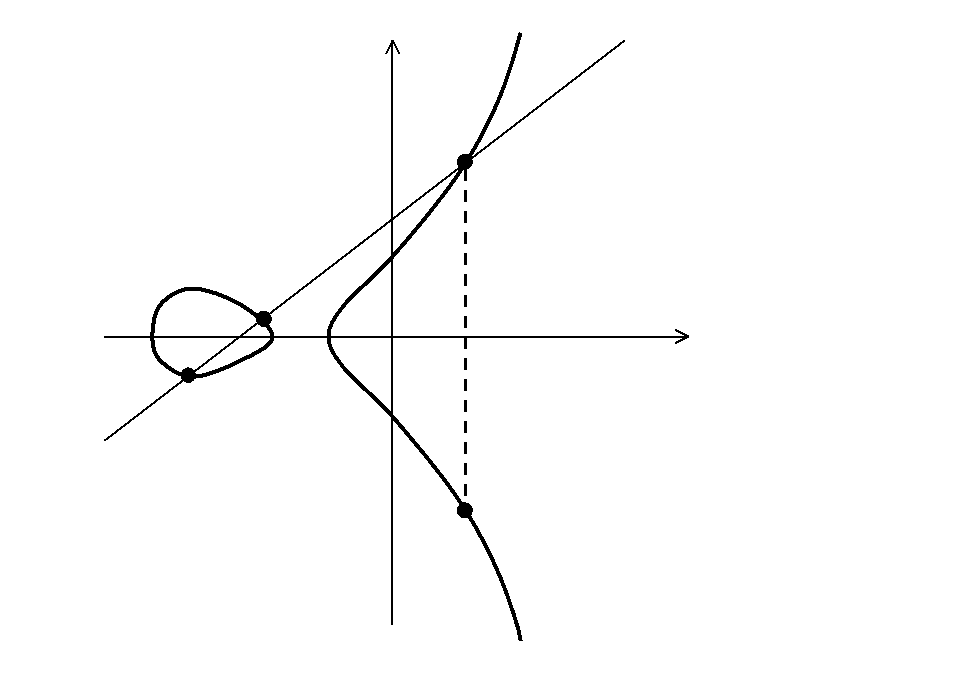
\includegraphics[width=0.6\textwidth]{eca.png}
\end{figure}

To prove that the points on the elliptic curve form an abelian group under the additive operation defined above, we need to show that it satisfies the three axioms: existence of inverses, commutativity, and associativity. The existence of inverse follows immediately from the definition since $(x,y) - (x,-y) = O$. Commutativity also follows from the definition as interchanging $P_1$ with $P_2$ does not make difference. However, showing the associativity requires deeper investigation of intersections of the curves which is beyond our scope.

\section{Discrete Logarithm Problem on E}
We have explored the algebraic structure of elliptic curves. It turns out this structure provides the reason why using elliptic curves permits us to use a smaller key size in approximately same degree of security. Similar to the original public key cryptosystem such as Diffie-Hellman or RSA, the elliptic curve cryptography relies on the discrete logarithm problem.
\begin{definition}
If $E$ is an elliptic curve over $F_p$ and $B$ is a point of $E$, then the discrete log problem on $E$ (to the base $B$) is the problem, given a point $P \in E$, of finding an integer $x \in \Z$ such that $xB = P$ if such an integer exists.
\end{definition}
It is known that the discrete logarithm problem over elliptic curve is harder to break compare to that over finite field. The main reason is the strongest techniques developed for the use in finite fields does not seem to work on elliptic curves because of its unique algebraic structure. In summary, If we avoid supersingular curves and curves whose order has no large prime factor, there is no known subexponential algorithm that breaks the system~\cite{Neal}. For example, Certicom, a company that strongly supports the elliptic curve cryptography, claims that an elliptic curve over $F_p$ where $p$ is $163$-bits is computationally infeasible~\cite{Stein}.

\section{Elliptic Curve Diffie–Hellman}
We now describe currently commonly used cryptography called Elliptic Curve Diffie-Hellman using the analogue between Alice and Bob. Suppose that Alice wants to send Bob an secrete message through an unprotected channel. They want to agree upon a secret key which will be used later for communication. To do that they first choose a finite field $F_p$ and an elliptic curve $E$ on it. Then, they publicly choose base $B$ which ideally have large order so that the subgroup generated by $B$ is very large. Next, Alice chooses secrete random integer $a$ of order of magnitude $p$. She computes $aB \in E$ and make it public. Bob does the same: chooses secrete random integer $b$, computes $bB \in E$, and make it public. The secret key they will use is $P = abB \in E$.

However, the third party knows only $aB$ and $bB$. Hence, without solving the discrete logarithm problem, there are no known ways to figure out what $P = abB$ is only knowing $aB$ and $bB$.

\bibliography{bib}{}
\bibliographystyle{plain}

\end{document}